\documentclass[tikz,border=7pt]{standalone}
\usepackage{amsmath}
\usetikzlibrary{arrows.meta,calc,positioning,decorations.pathmorphing}
\definecolor{ink}{HTML}{21352F}
\definecolor{teal}{HTML}{087F7B}
\definecolor{gold}{HTML}{C58B2A}
\definecolor{blue}{HTML}{4B77A8}
\definecolor{rose}{HTML}{B65A62}
\definecolor{paper}{HTML}{FFFCF6}
\begin{document}
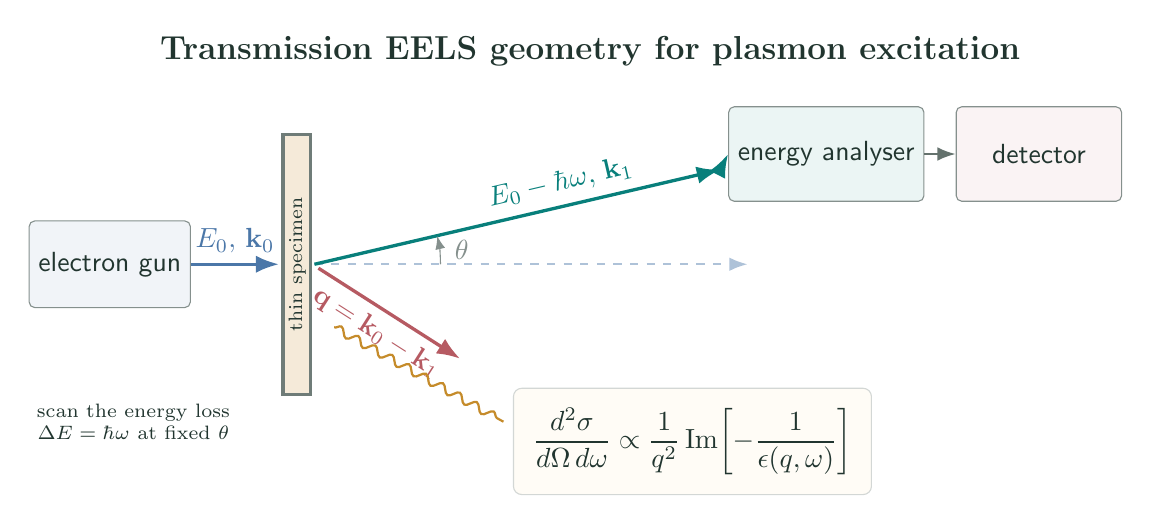
\begin{tikzpicture}[font=\sffamily,text=ink,>=Latex]
  \node[font=\bfseries\large] at (0,3.25) {Transmission EELS geometry for plasmon excitation};
  \node[draw=ink!55,rounded corners=2pt,fill=blue!8,minimum width=2.0cm,minimum height=1.1cm] (gun) at (-6.1,0.55) {electron gun};
  \draw[->,blue,very thick] (gun.east)--(-3.95,0.55) node[midway,above] {$E_0,\,\mathbf k_0$};
  \draw[ink!65,very thick,fill=gold!18] (-3.9,-1.1) rectangle (-3.55,2.2);
  \node[rotate=90,font=\scriptsize] at (-3.72,0.55) {thin specimen};
  \draw[->,blue!45,thick,dashed] (-3.5,0.55)--(2.0,0.55);
  \draw[->,teal,very thick] (-3.5,0.55)--(1.65,1.75) node[pos=.62,above,sloped] {$E_0-\hbar\omega,\,\mathbf k_1$};
  \draw[->,rose,very thick] (-3.45,0.5)--(-1.65,-0.65) node[midway,below,sloped] {$\mathbf q=\mathbf k_0-\mathbf k_1$};
  \draw[->,ink!55] (-1.9,0.55) arc[start angle=0,end angle=13,radius=1.6] node[midway,right=2pt] {$\theta$};
  \node[draw=ink!55,rounded corners=2pt,fill=teal!8,minimum width=2.3cm,minimum height=1.2cm] (ana) at (3.0,1.95) {energy analyser};
  \draw[->,teal,very thick] (1.65,1.75)--(ana.west);
  \node[draw=ink!55,rounded corners=2pt,fill=rose!7,minimum width=2.1cm,minimum height=1.2cm] (det) at (5.7,1.95) {detector};
  \draw[->,ink!70,thick] (ana.east)--(det.west);
  \draw[decorate,decoration={snake,amplitude=1.5pt,segment length=7pt},gold,thick] (-3.25,-0.25)--(-1.1,-1.45) node[right,font=\scriptsize,text=ink] {longitudinal density oscillation};
  \node[draw=ink!20,rounded corners=3pt,fill=paper,align=center,inner sep=7pt] at (1.3,-1.7) {$\displaystyle \frac{d^2\sigma}{d\Omega\,d\omega}\propto\frac{1}{q^2}\operatorname{Im}\!\left[-\frac{1}{\epsilon(q,\omega)}\right]$};
  \node[font=\scriptsize,align=center] at (-5.8,-1.45) {scan the energy loss\\$\Delta E=\hbar\omega$ at fixed $\theta$};
\end{tikzpicture}
\end{document}
